\chapter{Hybrid Ray tracer}
\label{chapter:hybrid}
%----------------------------------------------------------------------------------------
%	HYBRID RAY TRACER	
%----------------------------------------------------------------------------------------
Radio waves get simulated within the NuRadioMC framework via geometrical
optics, also known as ray tracing which we explained in section \ref{sec:WaveProp}.
The ray tracing algorithm that's being used is radiopropa and is dependent on
the ice model. To simulate a path using radiopropa you need a start position 
and a launch angle, if you only have the initial and final position you'll need
a wrapper algorithm for determining the launch angle.  
A wrapper algorithm that works with complex ice models was developed previously
called the \textit{iterative ray tracer}\cite{2022icrc.confE1027O}, and was
discussed in section \ref{sec:Iterative}.

The way the iterative ray tracer works is sub-optimal as it uses its own
procedure in python which in general will work slower and less accurate than an
optimization library. Work had been done on trying to implement an algorithm
using optimization libraries deemed the "minimizer", but this attempt failed as
there was no reliable way to determine initial launch angle intervals over
which to minimize.  As we saw this work, the idea came to mind to combine the
iterative ray tracer and the code used in this minimizer. Inspired, we
built the algorithm which will be discussed in this chapter: The \textit{hybrid ray
tracer}, in the source code called the "hybrid minimizer" \cite{hybrid}. 

The hybrid ray tracer succeeds in more rapidly finding the path from the event
to the detector than the iterative ray tracer, is also more accurate and
arrives closer to the detector as the final result is not limited by the final
drawn sphere size but by a given tolerance, making it useful for simulations in
which high time and space precision is needed like plane wave reconstruction,
which we'll do in chapter \ref{chap:WB}.

\section{How the hybrid ray tracer works}
The hybrid minimizer can be seen as an extension of the iterative ray tracer as
it starts out the same way, so to understand the first step I refer to section 
\ref{sec:Iterative}. Only the leftmost step of the three steps shown in figure
\ref{fig:IterativeWorkings} is completed, after this step two distinct launch regions
have been found.

After 2 distinct launch regions have been found, say in the regions
$[\theta_1,\theta_2]$ and $[\theta_3,\theta_4]$, 
then the so called \textit{minimization} procedure will
start. Using scipy's module optimize.minimize the optimal solution will be
found by using the Nelder-Mead method\cite{10.1093/comjnl/7.4.308}. First we
get rid of the spherical observer and place the vertical observer at the
detector, now to be able to use the minimize module we'll need a function to
minimize, for this reason we first define the function \textit{delta\_z} as,
given a certain launch angle, propagating the ray onto the vertical observer
and returning the distance from the point where it lands on the plane to the
detector, as illustrated on figure \ref{fig:PrincipleHybridIllu} (i.e it
returns the value $\Delta z$).
\begin{figure}
  \centering
  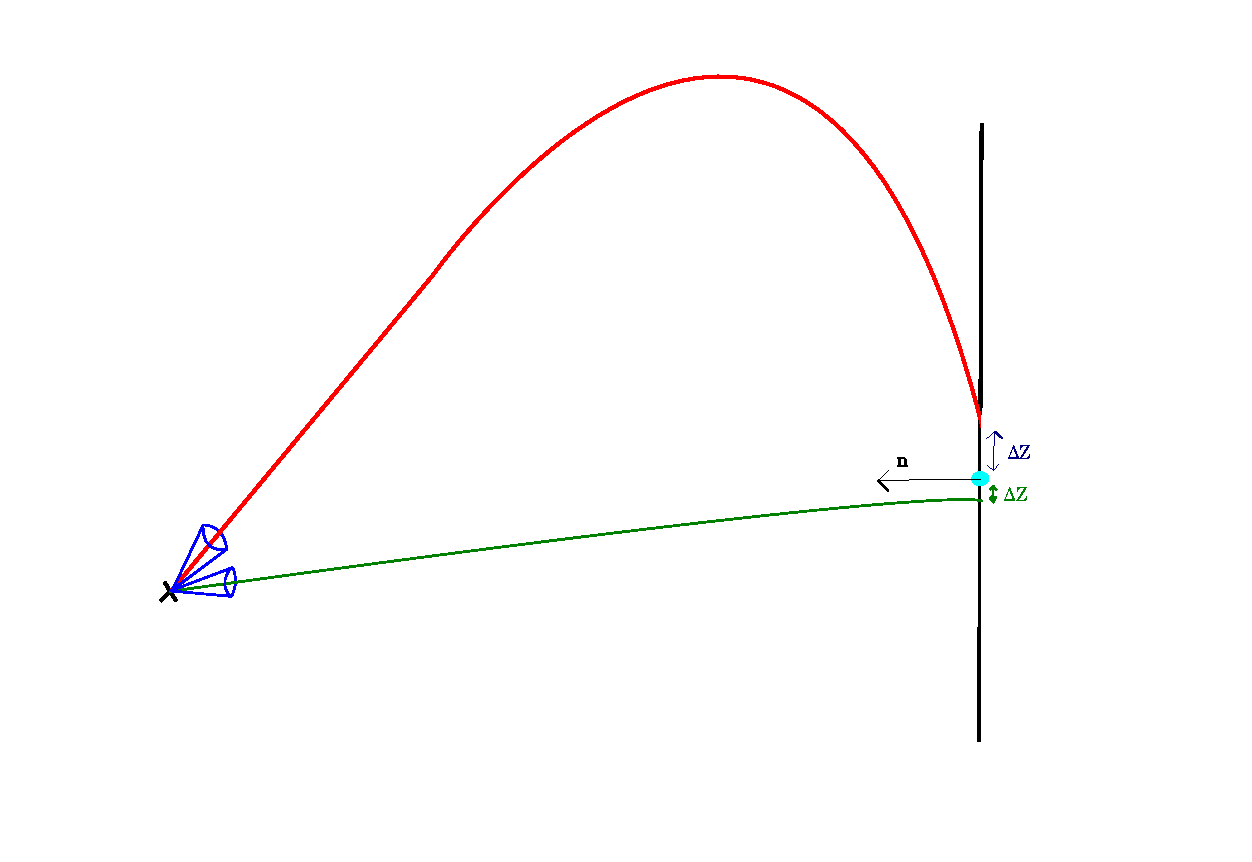
\includegraphics[width=0.7\textwidth]{PrincipleHybridIllu.pdf}
  \caption{The algorithm shoots rays in a direction within the blue cone angle intervals and minimizes the $\Delta z$ that gets returned}
  \label{fig:PrincipleHybridIllu}
\end{figure}
The function we'll minimize is then delta\_z\_squared which just squares the
value which delta\_z returns as we want to minimize to zero. 
We use the previously found angle boundaries as
the boundaries for this minimization algorithm, meaning that if the 2 zenith
angle intervals $[\theta_1,\theta_2]$ and $[\theta_3,\theta_4]$ were found in
the first step of the algorithm it will first minimize $\Delta z^2$ within the
first angle interval and find its solution and then within the second angle
interval. With this our algorithm is done, it does have a fail-safe as well in case
that the first step, finding the launch regions, doesn't find the 2 launch
regions.  Namely it reverts back to being the iterative ray tracer.

\section{Performance Optimization} 
We wish to optimize this algorithm to make
it as fast as possible.  To consistently test the algorithm after every
particular change in a parameter, we'll be randomly generating vertex
interaction positions keeping the detector at the fixed location of (0,0,-100).  To
this end the numpy random module was used to generate random coordinates. The
considered square (as there is only a z component to the ice model, the 3D
problem has cylindrical symmetry and thus essentially only a 2D problem) is
x:0.1km,4km and z:-0.1km,-3km\footnote{This start at 100m depth was to get
around issues concerning events that won't even trigger in a full simulation}.
Every simulated point shown in the following subsections consists of at least
500 random initial positions.  As the speed of the algorithm is computer
dependent, the algorithm's speed is always plotted relative to the iterative ray
tracer's speed, simulated with the same coordinates and under equal computer load.

Now we don't just want to achieve higher speed in our algorithm, we also want
to at least have the same accuracy as the iterative ray tracer, if not even better.
To this end we need to check with an "exact solution". There is only one candidate
that fits this role: \textit{the analytic ray tracer}. The plan is thus to use the
exponential ice model as a testing ground for the hybrid ray tracer and solving each
vertex-detector ray tracing problem with both the iterative, analytic and hybrid ray tracer.
After having solved for the \textbf{propagation time} (meaning the time it takes the ray to
propagate from the source to the detector) and the \textbf{arrival zenith angle} (the zenith angle
the ray makes at the detector) for each of the algorithms we can infer the accuracy of a particular
algorithm by how much it differs from the solution found through the analytic ray tracer.
\subsection{Length of the normal vector}
\begin{figure}
	\centering
	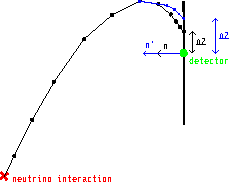
\includegraphics[width=0.6\textwidth]{figures/PrincipleNormIllu.pdf}
	\caption{the steps taken are illustrated with the dots, the spacing reduces close to the detector. Changing
	the normal vector changes the spacing and thus the accuracy.}
	\label{fig:normexpl}
\end{figure}
While figuring out what was wrong with the initial \textit{minimizer} we
stumbled on the fact that radiopropa has a weird little quirk.  As visually
explained in figure \ref{fig:normexpl}, the size of the normal vector seems to
influence how big radiopropa's ray tracer's step size is close to the
detector.  This thus influences the accuracy and total computational time
taken. The results of varying the length of this normal vector, comparing the
accuracy (in timing and arrival zenith) with the analytic ray tracer and the computational time with the
iterative ray tracer, are shown in figure \ref{fig:norminfl}.  
Looking at these figures we can make a first optimization
conclusion: as expected we should take the normal vector length to be 1 unit in radiopropa.
We can deduce this as the calculation speed seems to be minimal there 
and the accuracy drops rapidly after 1 meter.
Note that none of the measurements performed during this chapter have
error bars, this is because this optimization procedure is only to get
us roughly into the right ballpark.

\begin{figure}
	\centering
	\begin{minipage}{\textwidth}
		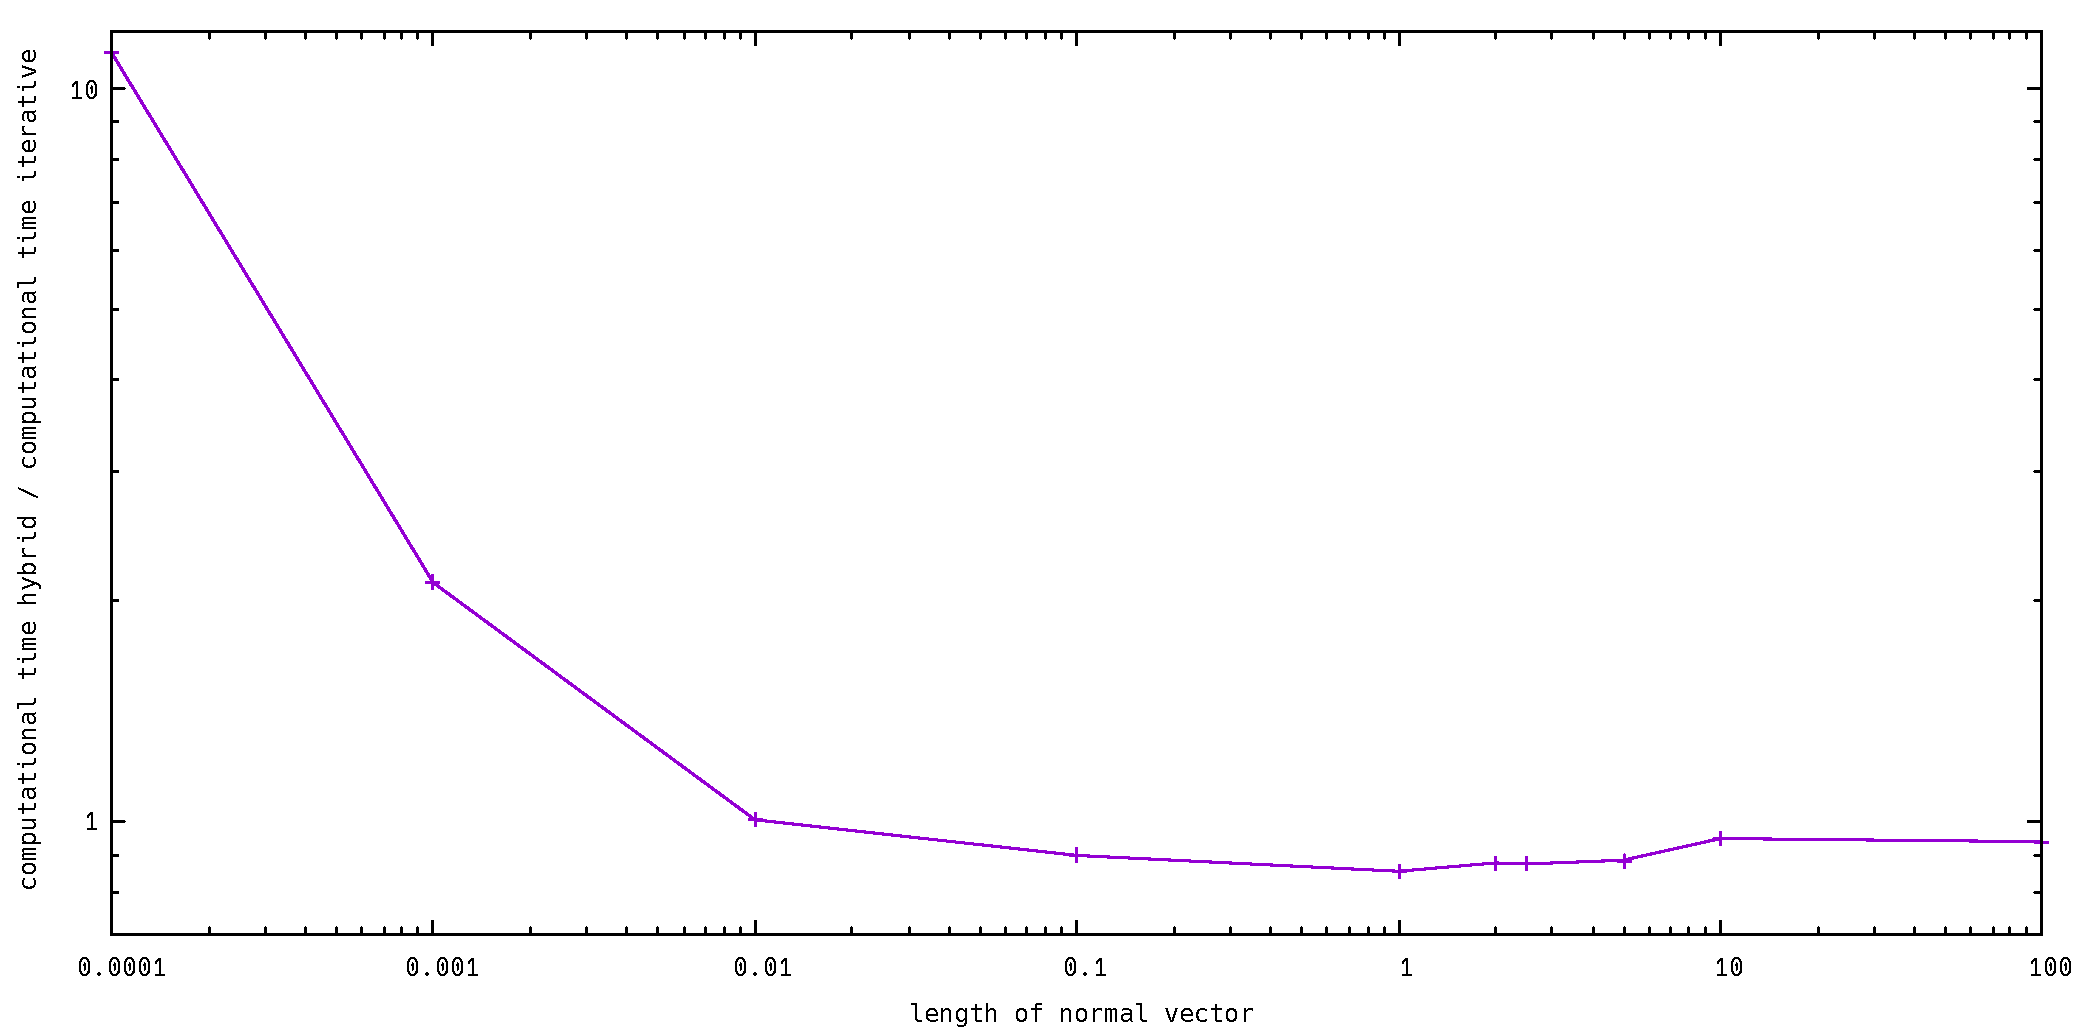
\includegraphics[width=0.9\textwidth]{figures/NormVsTime.pdf}
	\end{minipage}
	\begin{minipage}{\textwidth}
		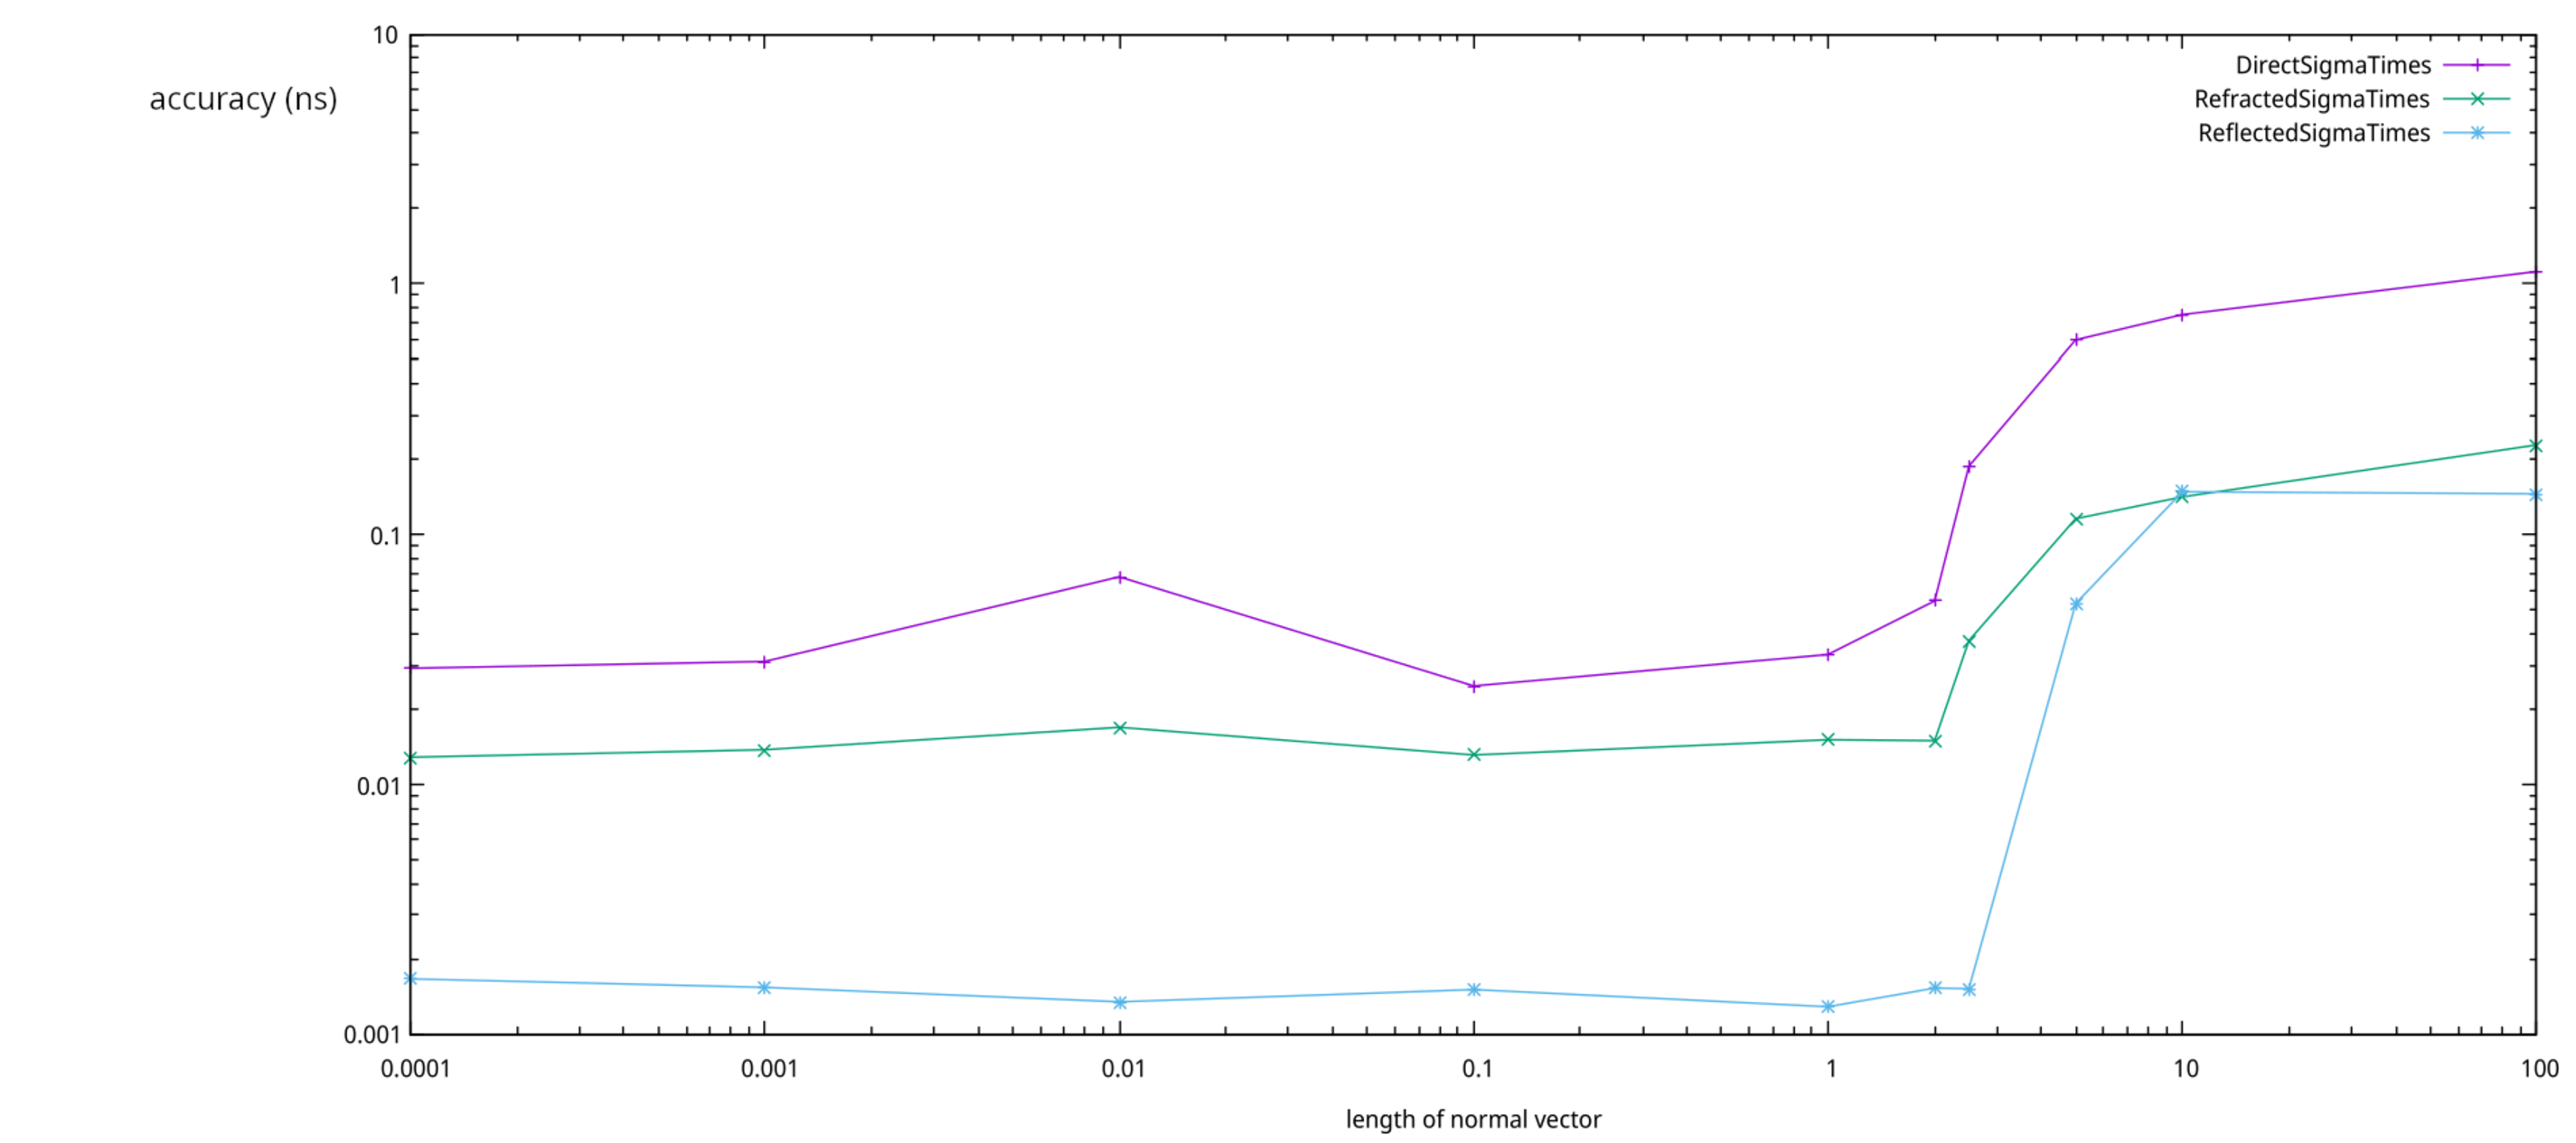
\includegraphics[width=0.9\textwidth]{figures/NormVsSigmaTime.pdf}
	\end{minipage}
	\begin{minipage}{\textwidth}
		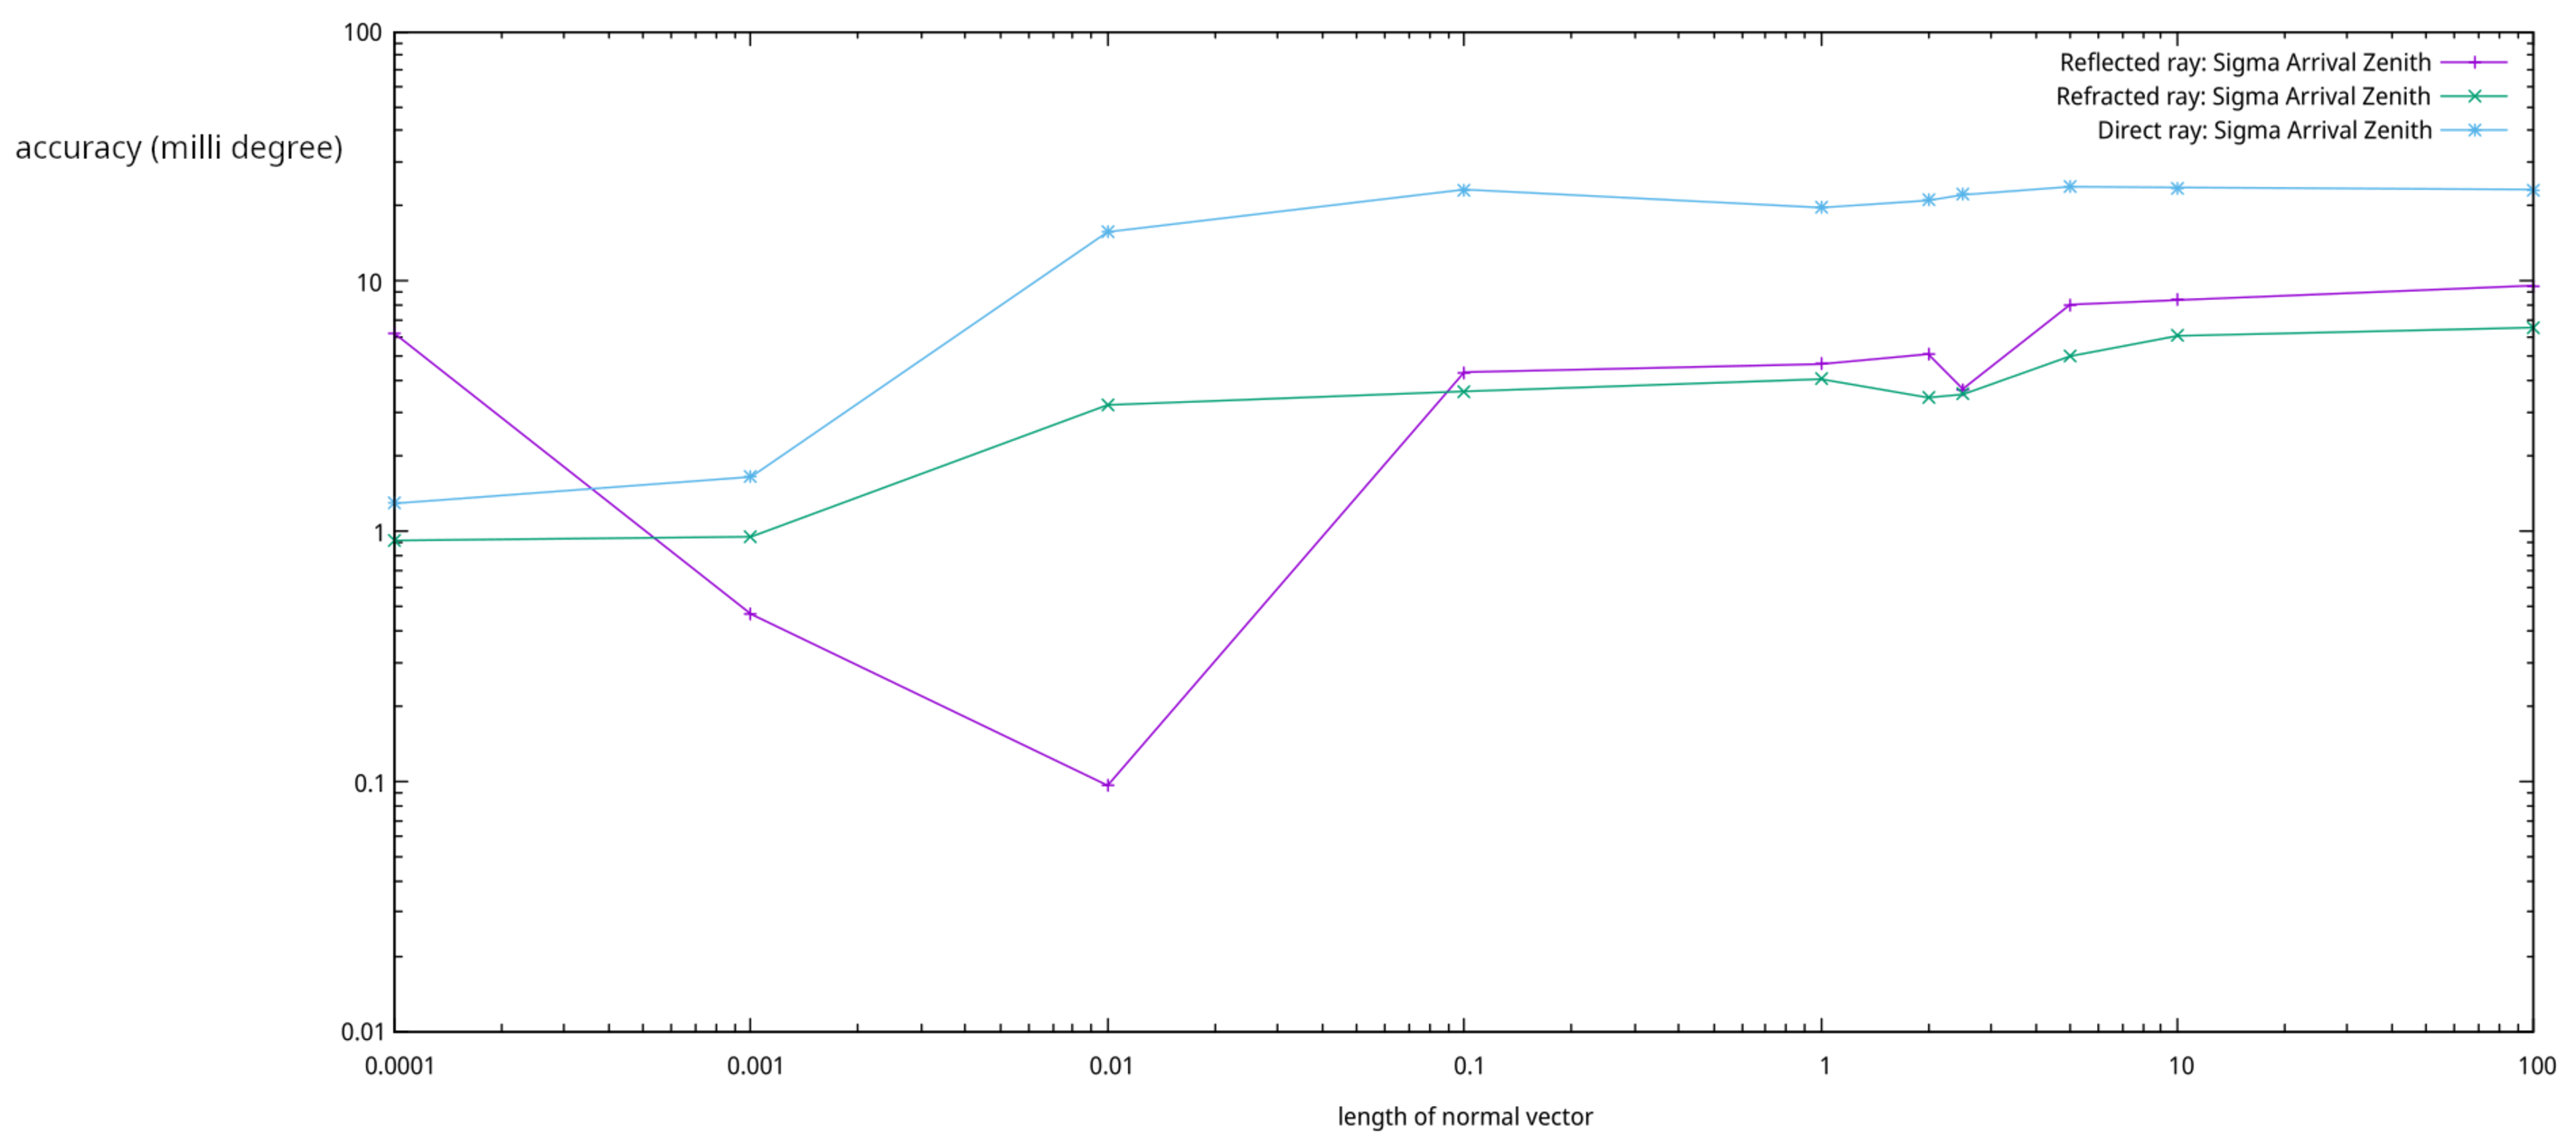
\includegraphics[width=0.9\textwidth]{figures/NormVsSigmaAZ.pdf}
	\end{minipage}
\caption{The speed first lowers with larger normal vector length, reaching a minimum near 1 but the accuracy in timing gets worse after a length of 1. We thus
conclude to take a normal vector length of 1.}
\label{fig:norminfl}
\end{figure}

\subsection{ztol}
We'll now change the \textit{tolerance}, with this we mean when 
the minimization algorithm returns a $\Delta z$ smaller than a certain
threshold "ztol" the ray will be accepted as the solution.  
The results from analogous comparisons as
previously discussed are shown in figure \ref{fig:ztolinfl}.
\begin{figure}
	\centering
	\begin{minipage}{\textwidth}
		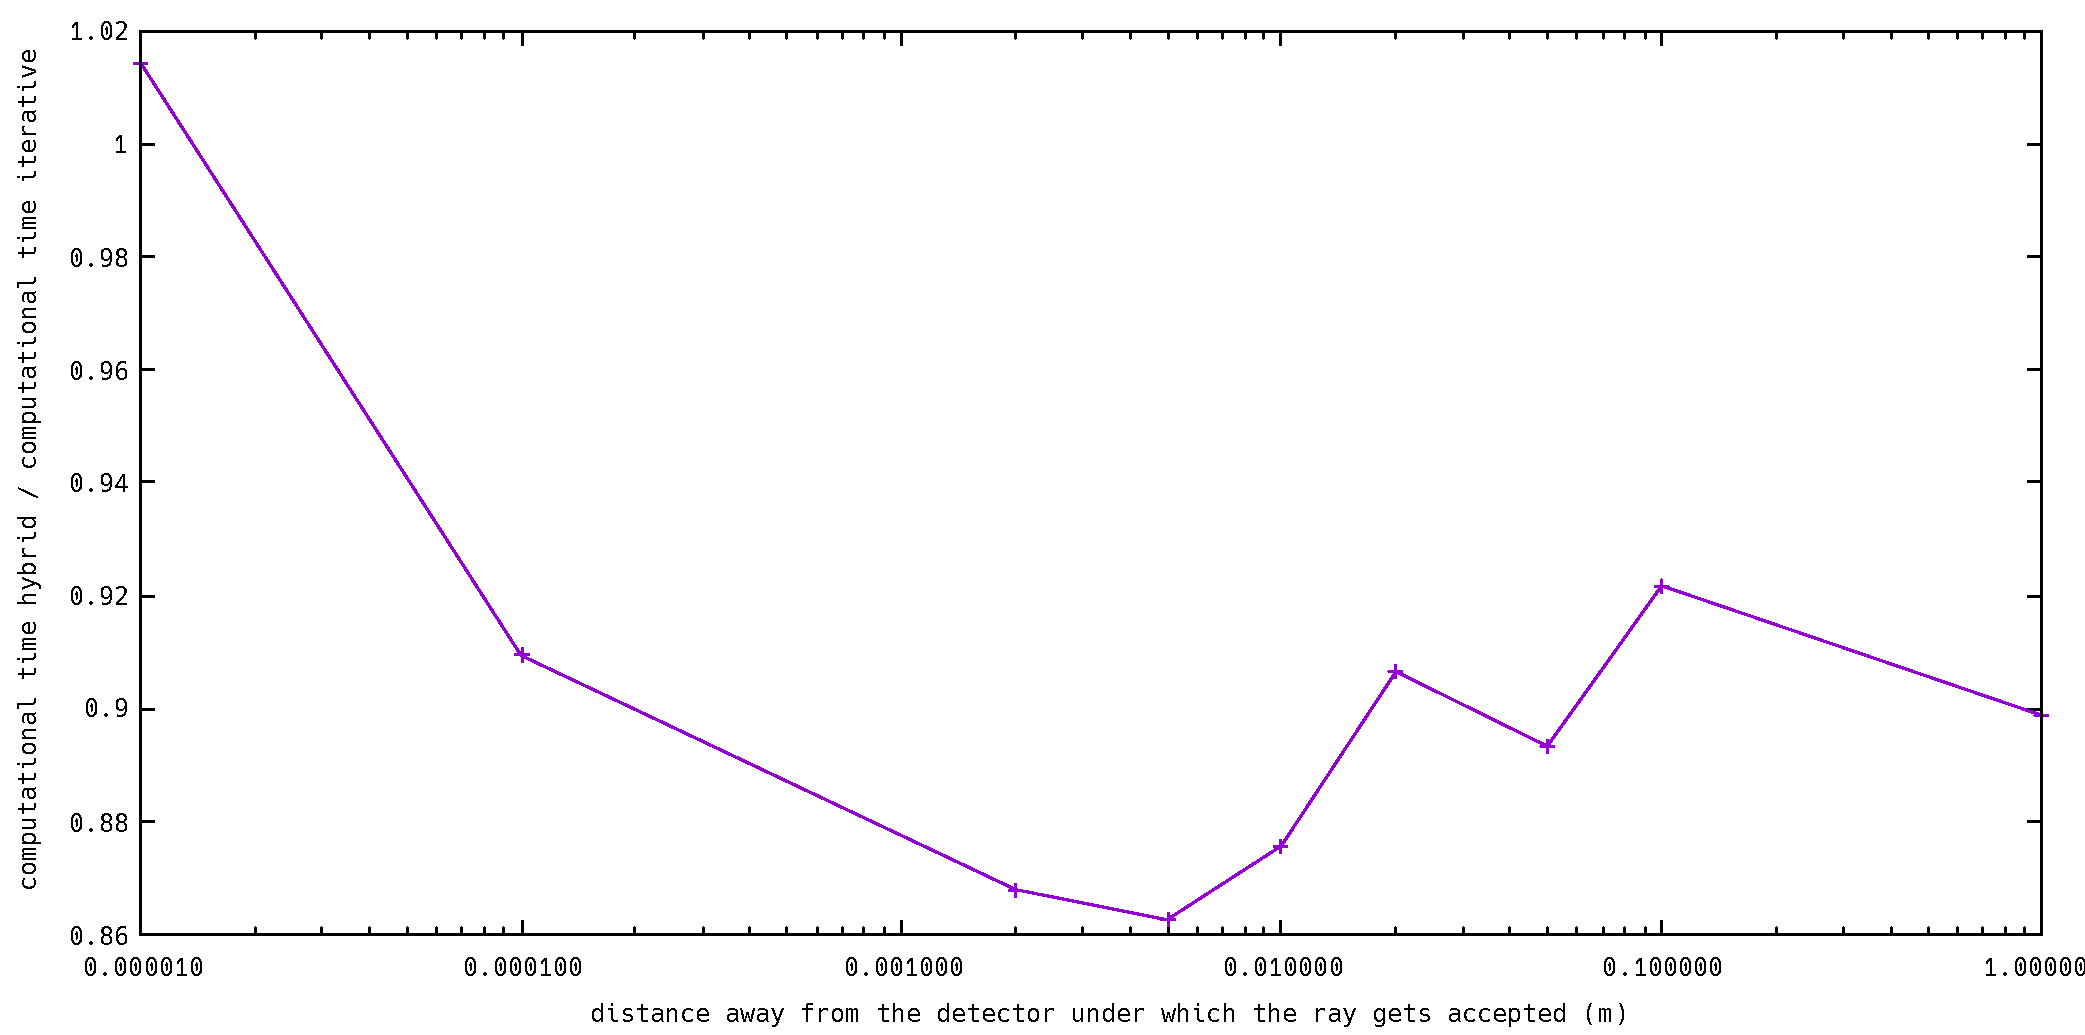
\includegraphics[width=0.9\textwidth]{figures/ZtolVsTime2.pdf}
	\end{minipage}
	\begin{minipage}{\textwidth}
		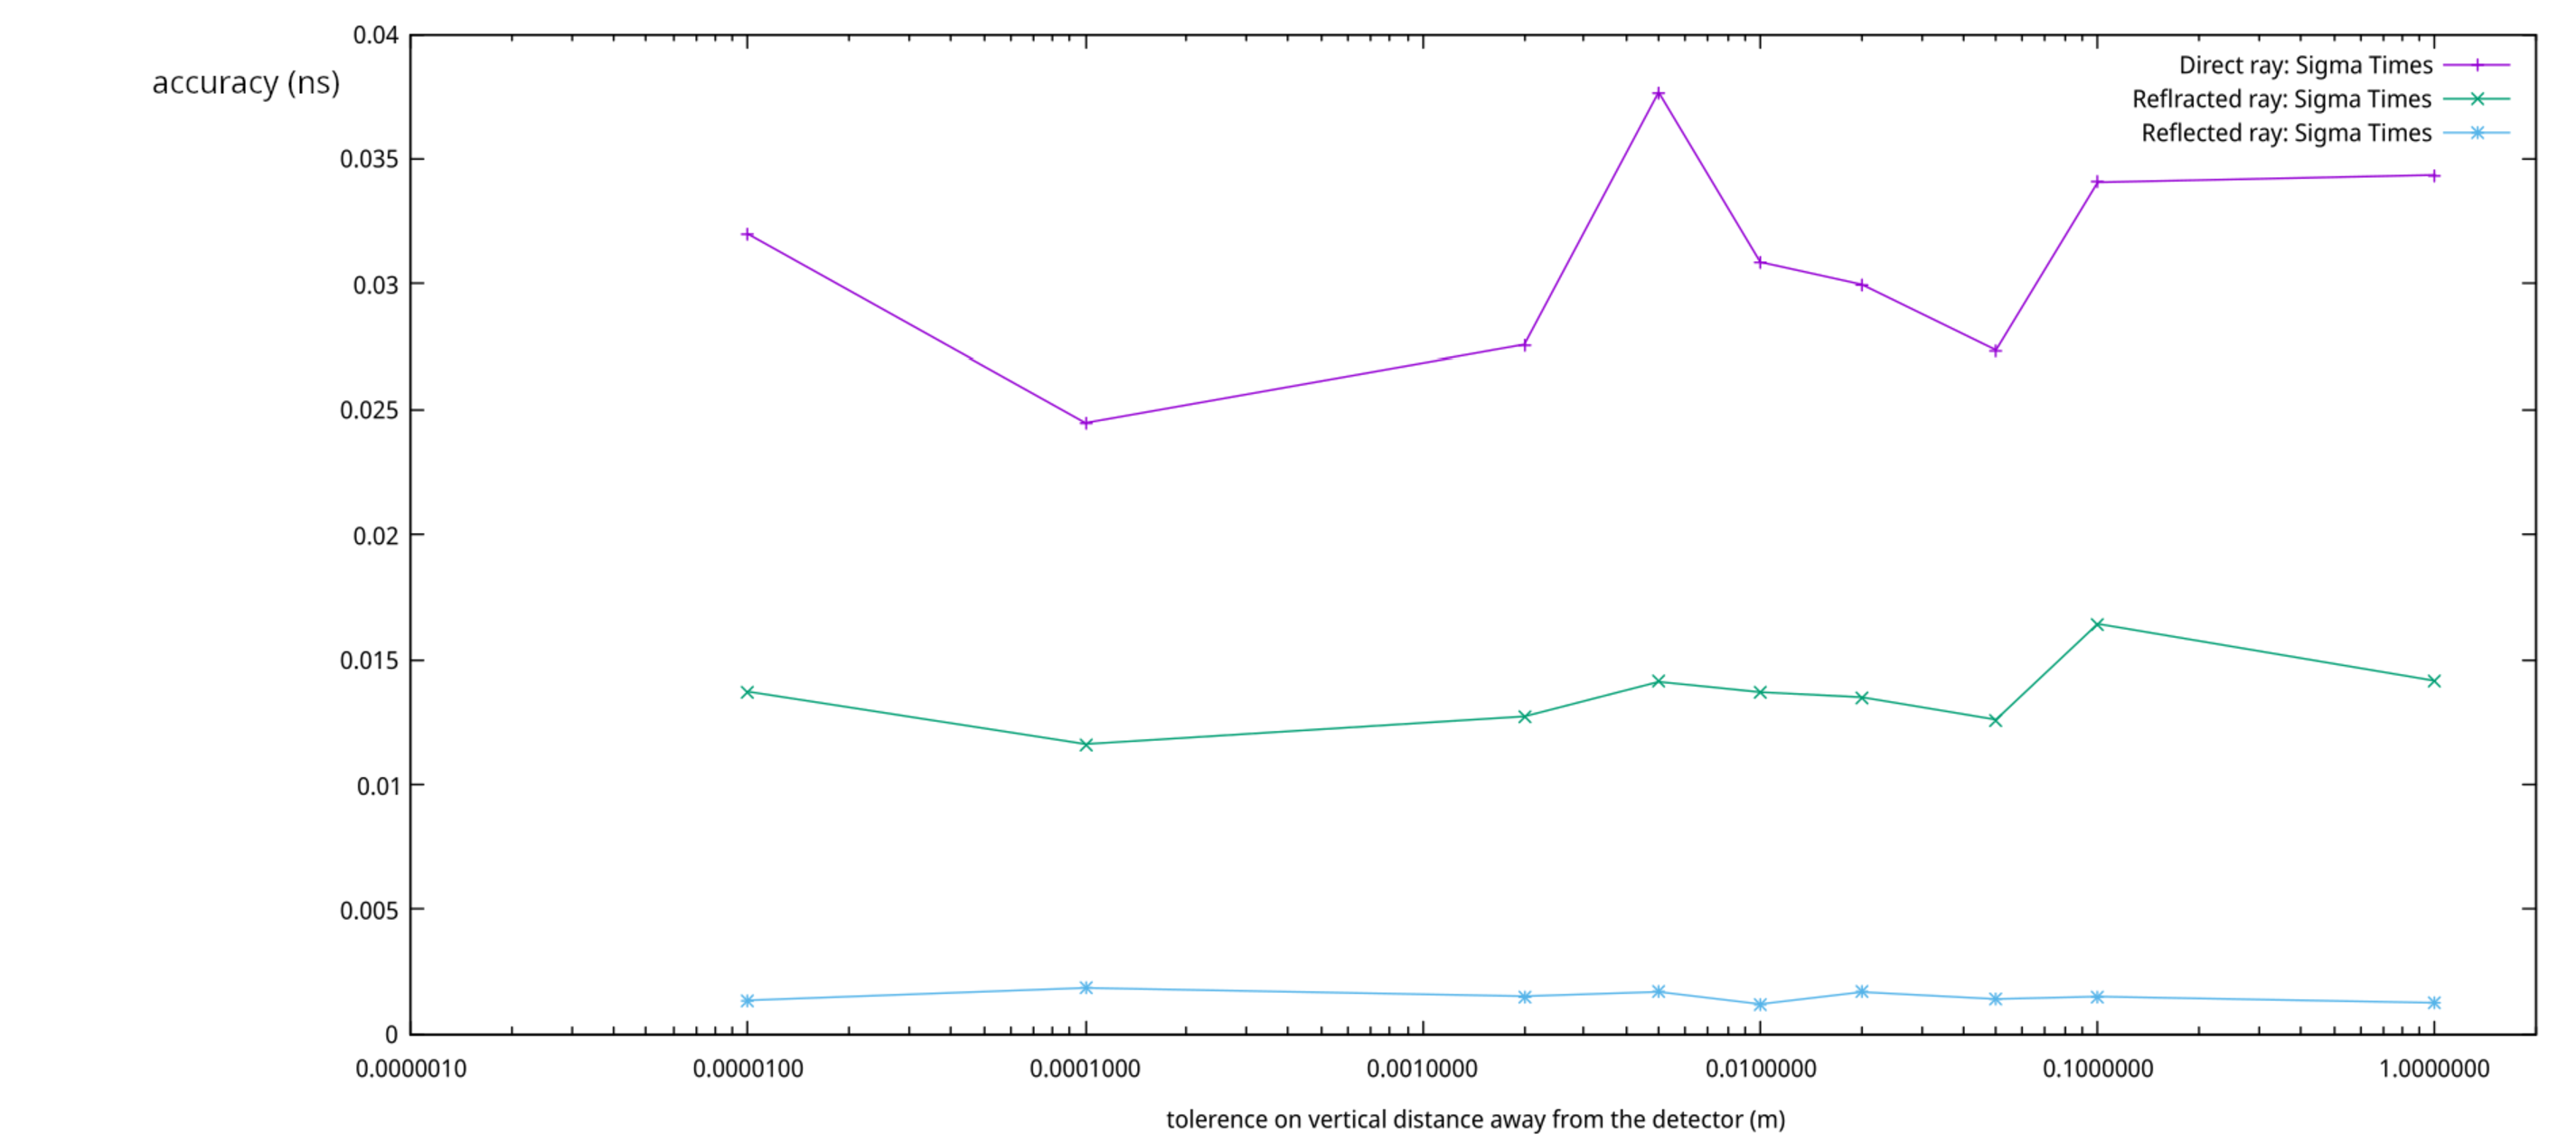
\includegraphics[width=0.9\textwidth]{figures/ZtolVsSigmaTime.pdf}
	\end{minipage}
	\begin{minipage}{\textwidth}
		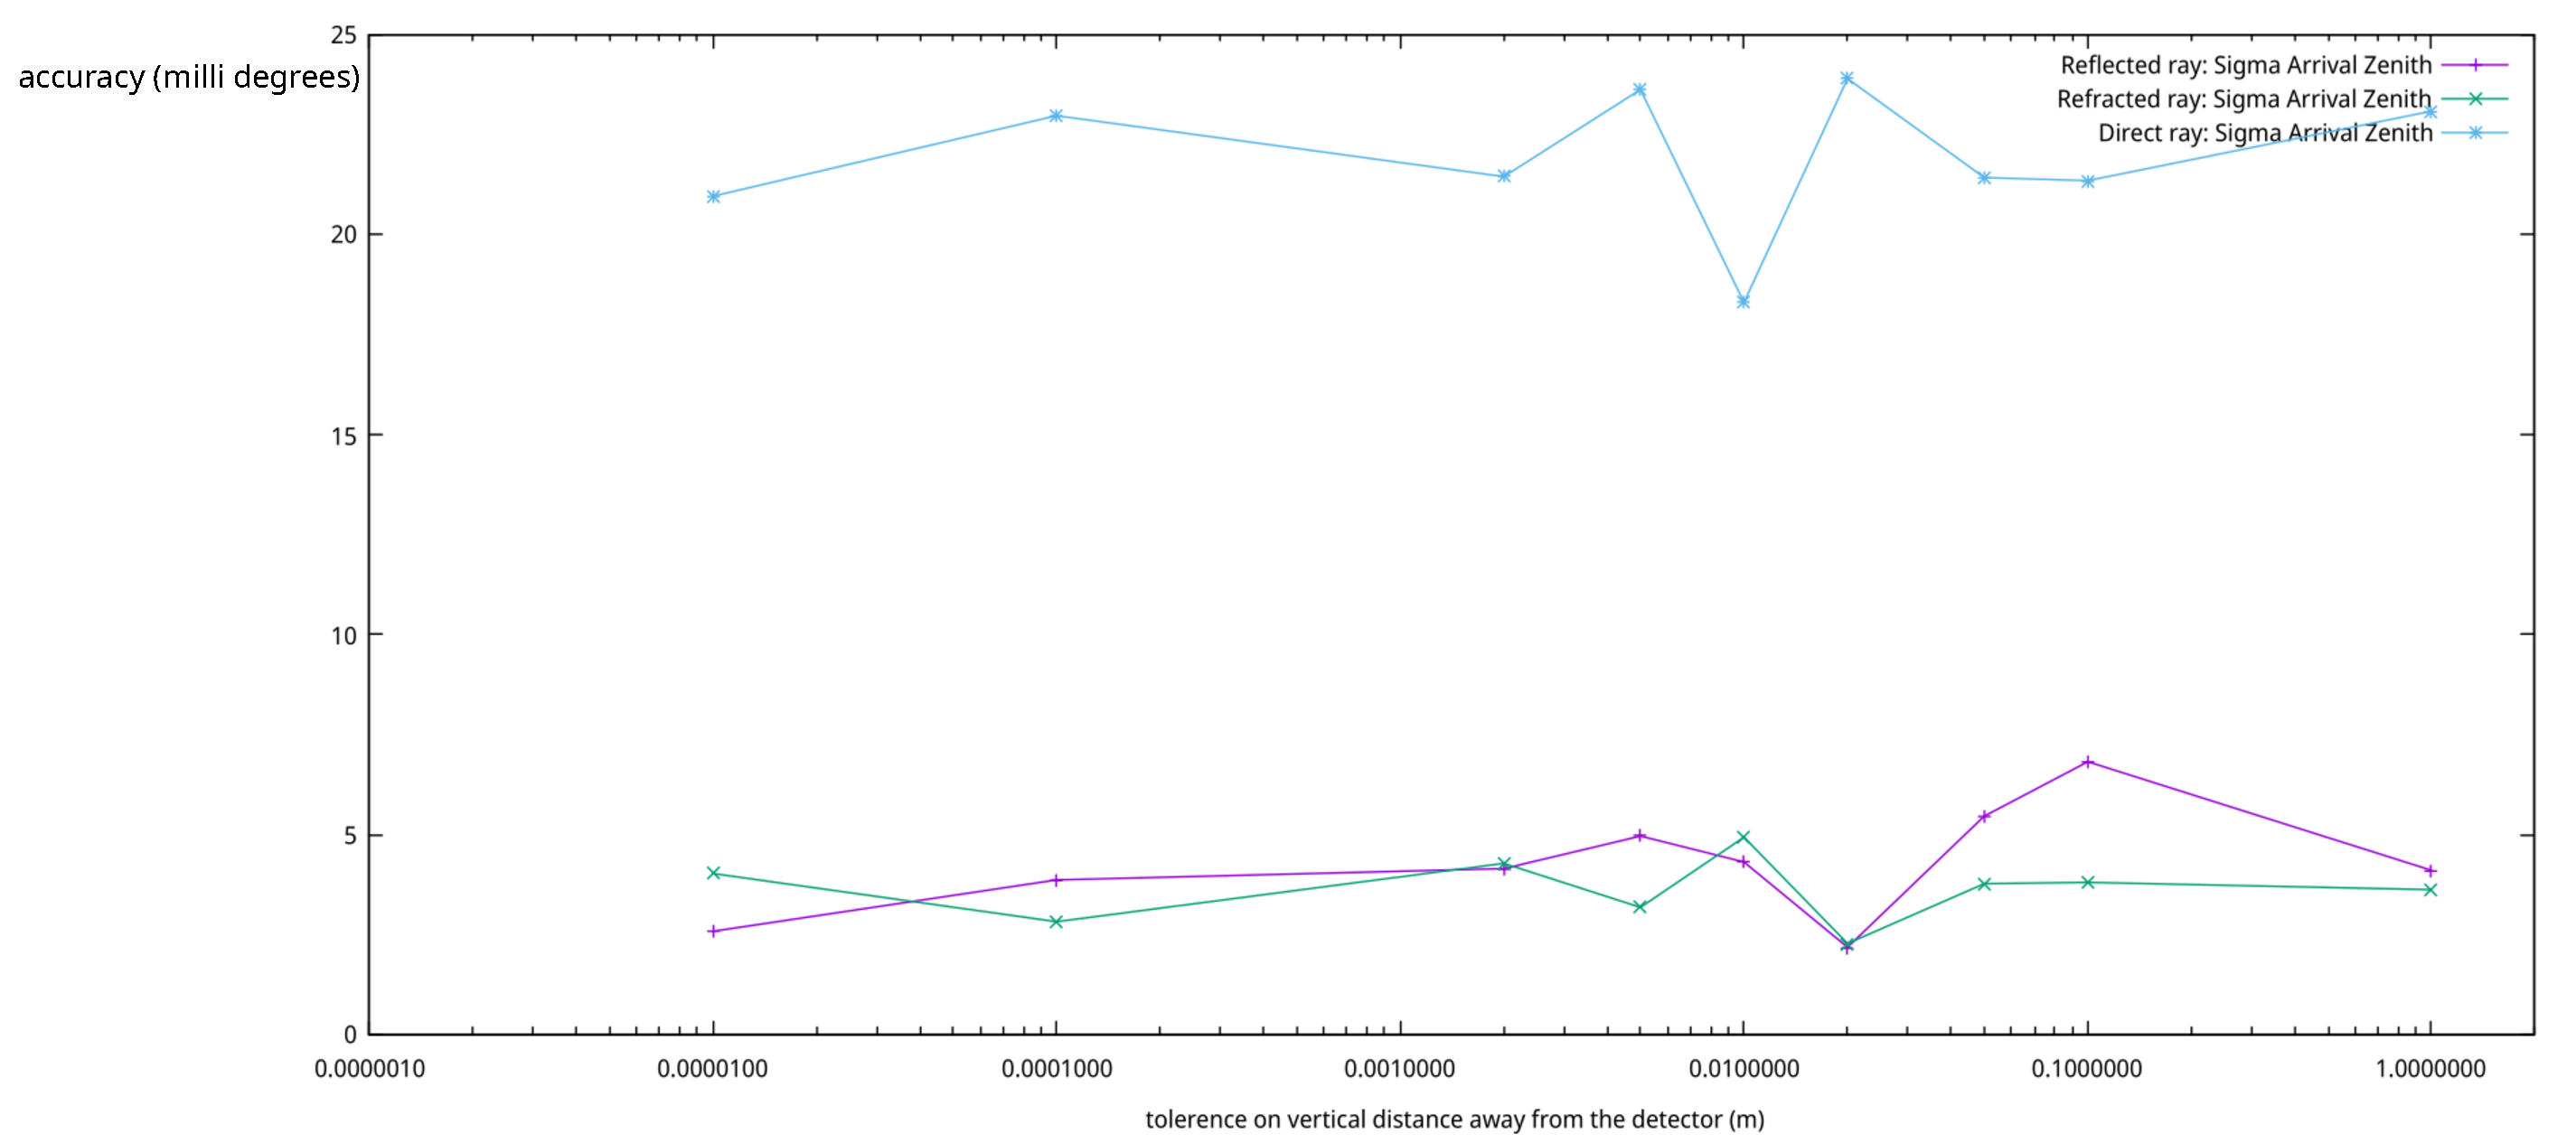
\includegraphics[width=0.9\textwidth]{figures/ZtolVsSigmaAZ.pdf}
	\end{minipage}
\caption{the solution seems to reach a minimal time at a tolerance of 5cm whilst both the accuracy in timing and the one on the zenith angle stay roughly the same, we thus conclude the zenith
tolerance to be 0.05m for optimal computing.}
\label{fig:ztolinfl}
\end{figure}
\newpage
There seems to be a minimum around 0.05m, looking at the
accuracy for this tolerance it seems sufficient to be used.  We can thus infer
the second optimization conclusion: take ztol to be 0.05 m.

\subsection{Sphere \& Step Size}
The initial rays are sent out in steps of a certain angle and with a sphere
around the detector of a certain size. Varying the parameters of this first
step of the algorithm (e.g the step size and sphere size) might thus have an
effect on both the accuracy and the computational time.  As this initial search
for launch angle regions is also the slowest step in the hybrid ray tracer (takes
$\approx 57\%$ of the total computation time)
it's also the most important step to optimize. The optimization procedure is as
follows: change the sphere size and loop over various step sizes, recording the
speed. Note that, as we have to vary 2 parameters, we can't really look at
accuracy here. This isn't needed however as we'll see that after finding the
optimal solution the accuracy is still sufficient. However, one thing we need to
keep an eye on is that during the optimalization there are always sufficient solutions found. 

As we wish this algorithm to be better than the iterative ray tracer, it'll
need to find at least as many solutions as the iterative ray tracer does.  If,
for a particular random interaction vertex location, less solutions are found
by the hybrid ray tracer than for the iterative ray tracer, this parameter
choice will be thrown away (and colored differently).  The results are shown in
figure \ref{fig:SphereStepInfl}, the points colored red are unusable following
the previously discussed criterion of sufficient solutions.  Looking at the
lowest green point (circled in blue), we see that an optimal sphere size seems
to be at 45m accompanied by a step size of 0.7°, this is in contrast to the
iterative ray tracer where a sphere size of 25m and stepsize of 0.5° is used.
Note that changing these values for the iterative ray tracer doesn't change its
speed nor accuracy.
\begin{figure}
\centering
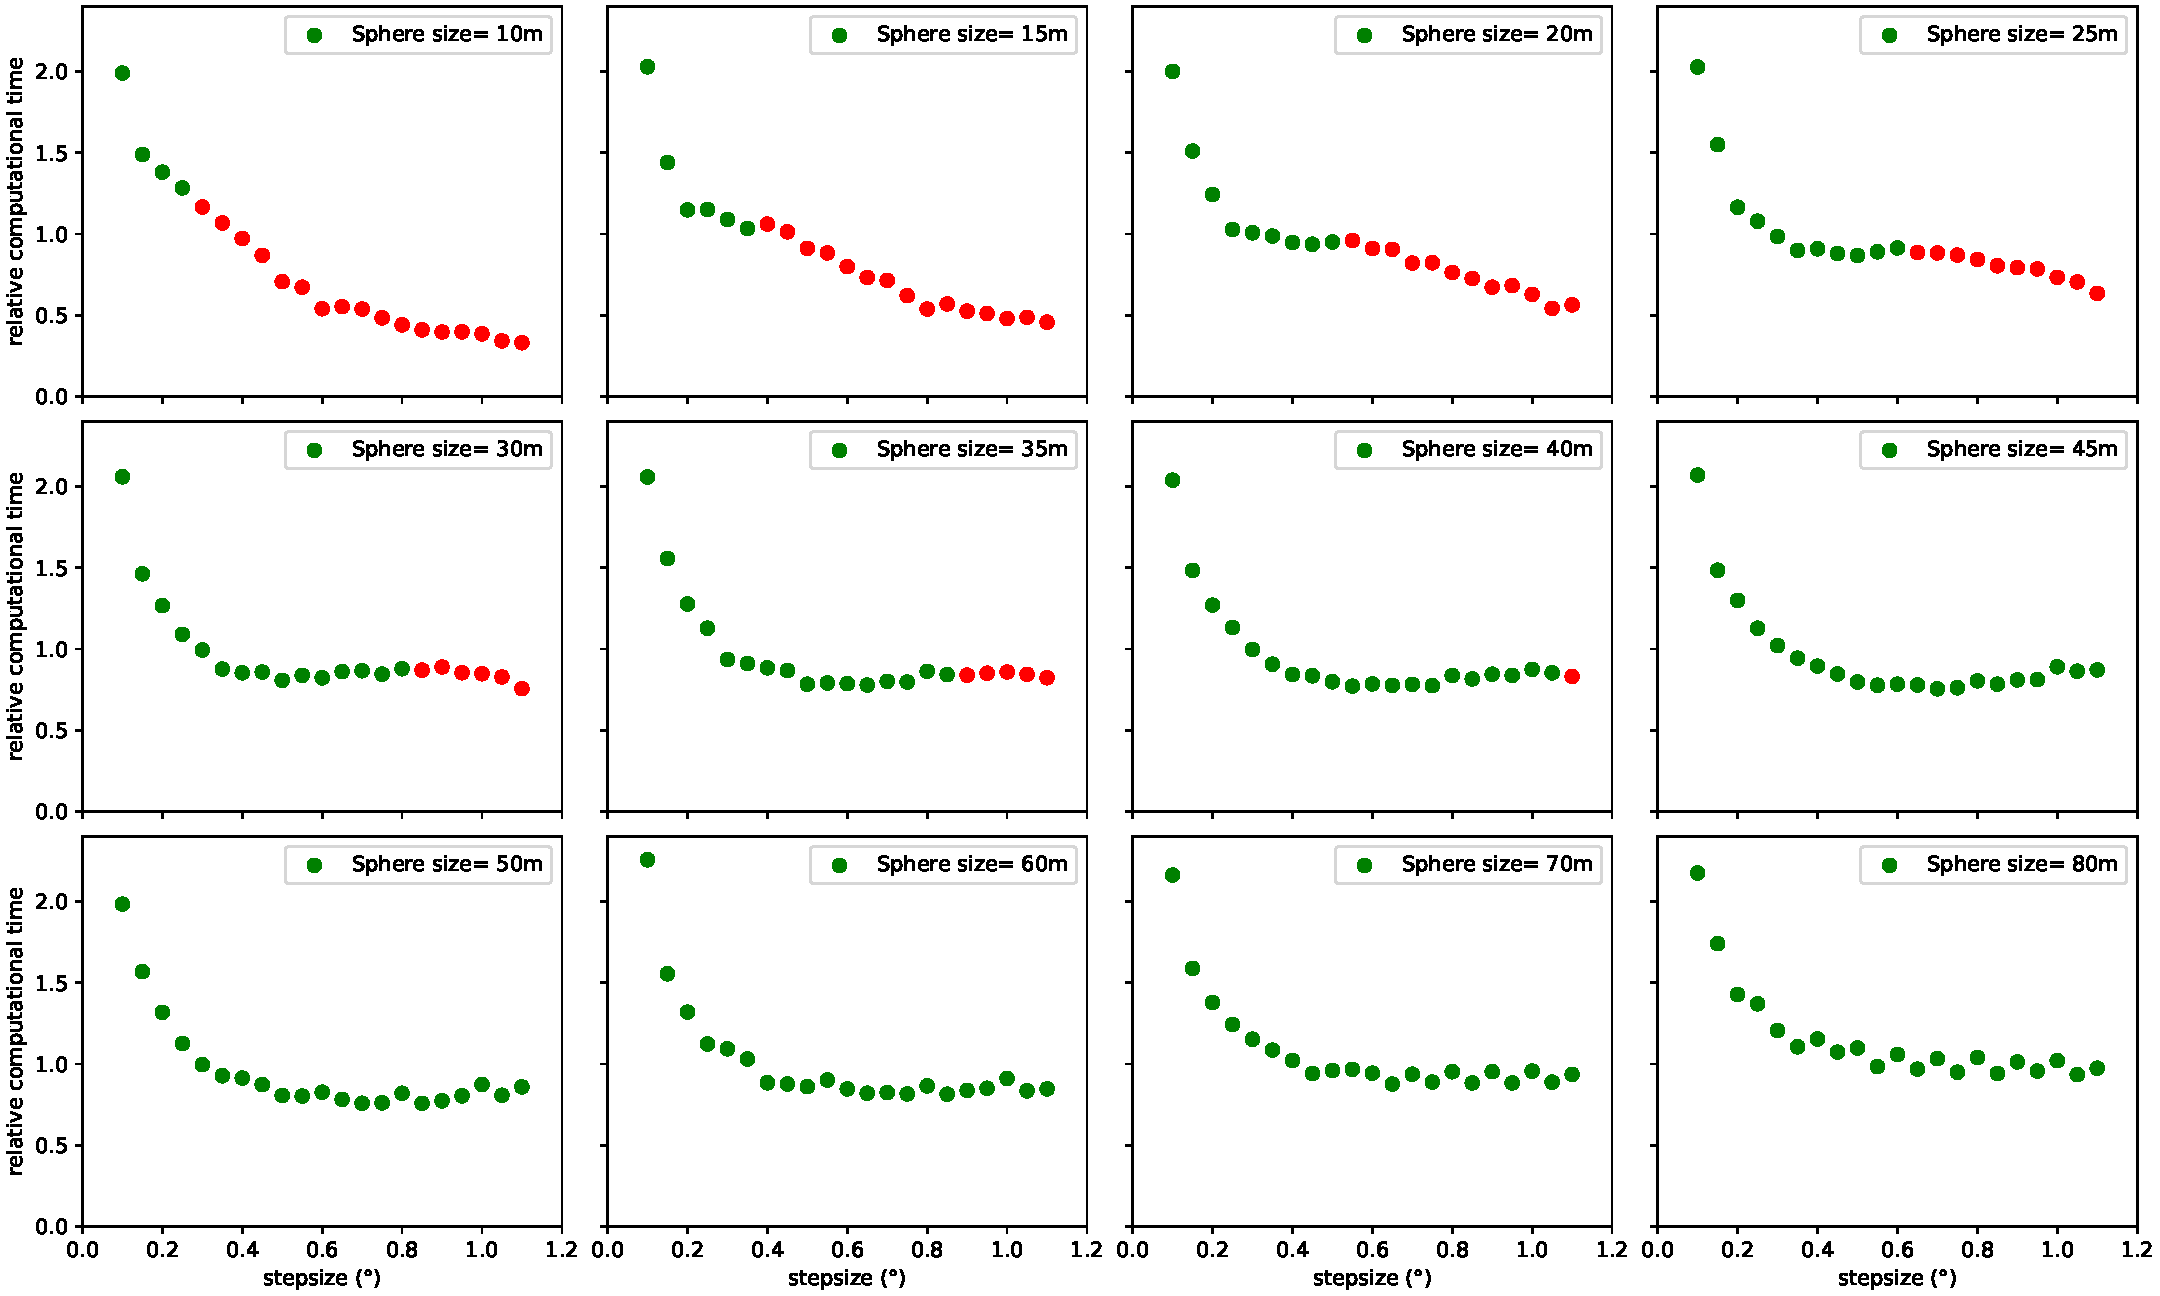
\includegraphics[width=\textwidth]{figures/subplotofallstepsphere.pdf}
\caption{The data in green is acceptable. At high sphere size the geometric effects start to play a role and staggering is observed. Circled in blue is the fastest setting which is also acceptable: 
0.7° angle stepsize and a spheresize of 45m}
\label{fig:SphereStepInfl}
\end{figure}
\subsection{Conclusion of optimization}
How does the hybrid ray tracer perform relative to the iterative ray tracer if we use 
the previously optimized variables? After doing a simulation of 1000 random source locations (double the previous amount) with
the iterative, analytic and hybrid ray tracer and comparing both the iterative and hybrid to the analytic 
we get what's shown in figures \ref{fig:acchyb} and \ref{fig:accit}. Where we can clearly see that the hybrid
ray tracer is more accurate. During this simulation we also recorded the computational speed, the fractional
speeds relative to the analytic ray tracer are presented below:
\begin{itemize}
	\item iterative: $5.93 \times 10^{-5}$ computations/analytic computation
	\item hybrid: $7.97 \times 10^{-5}$ computations/analytic computation
\end{itemize}
The hybrid ray tracer is thus 33.7\% faster than the iterative ray
tracer. The speed difference with the analytic ray tracer might seem
quite overwhelming but this can get mitigated in the future if part
of the hybrid ray tracer gets rewritten in a compiled language
like C++ in which the analytic ray tracer was written.

\begin{figure*}
	\centering
\begin{minipage}{0.49\textwidth}
	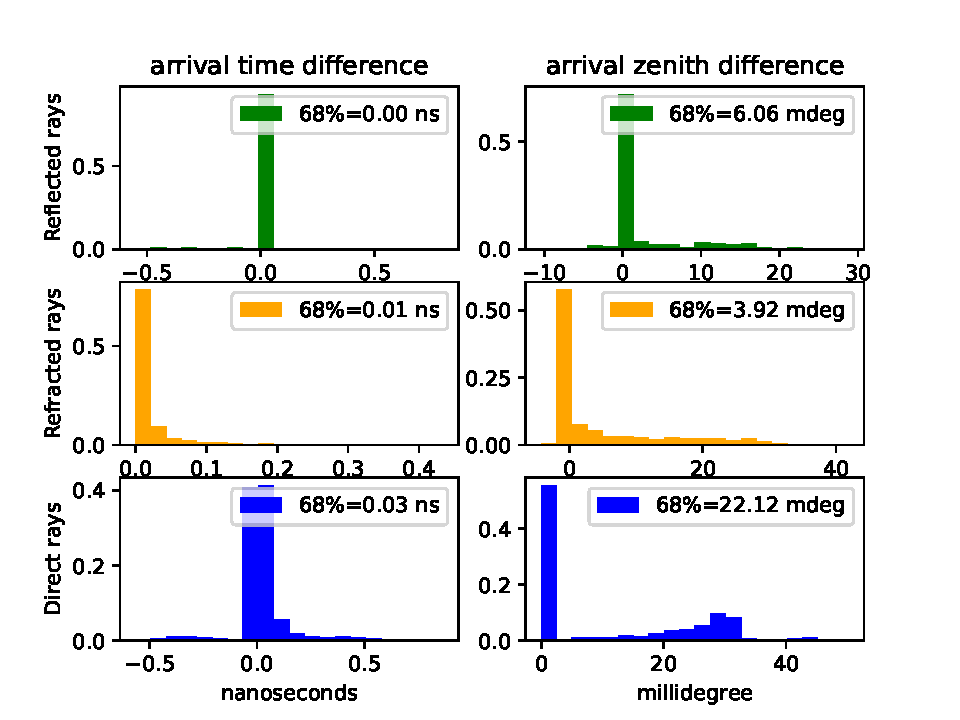
\includegraphics[width=1.1\textwidth]{figures/hybrid_comparison_N_1000.pdf}
	\caption{Accuracy of the hybrid ray tracer}
	\label{fig:acchyb}
\end{minipage}
\begin{minipage}{0.49\textwidth}
	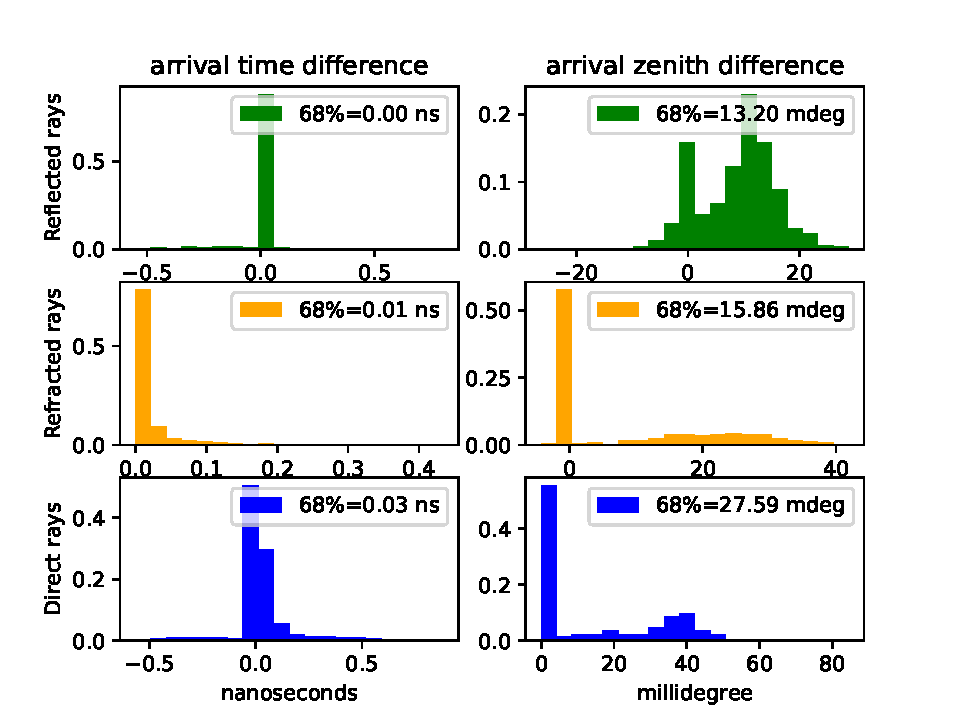
\includegraphics[width=1.1\textwidth]{figures/iterative_comparison_N_1000.pdf}
	\caption{Accuracy of the iterative ray tracer}
	\label{fig:accit}
\end{minipage}
\end{figure*}


